
\section{Our Novel Profitability Analysis}

\subsection{Realistic Code-Size Cost}

In Section~\ref{sec:deeplearning:motivation}, we describe the limitations of code size estimation using existing compiler's cost models.
In our motivation, we use an oracle cost model, with perfect information, that can be obtained by recompiling the whole program in order to decide which version produces a smaller binary.
However, this solution is infeasible due to compilation time overheads.
Large programs with thousands of functions can take days to optimise due to the excessive number of long recompilations, sometimes taking up to a couple days.

In this section, we propose a novel approach based on partial recompilation.
This approach is capable of significantly reducing the compilation time required by the oracle cost model, while still providing equivalent benefits.

%Our goal is to be able to capture the changes in the code that result from merging a pair of functions.
Our goal is to extract to a separate module only the code that can be potentially affected by merging a given pair of functions.
Beyond the difference in size of the merged function itself, code size can also be affected by the need for a thunk that calls the merged function while preserving the original interface.
Call-sites updated to call the merged function require extra arguments which might affect code-size directly or indirectly. %%i.e., higher register pressure
Finally, inter-procedural analyses and optimisations can have their decision making altered by the merged function.

In order to capture all the possible ways that function merging can influence code size, we extract to a different module the functions being merged as well as their user functions, such as callers or functions that take their address.
We also need to extract all global definitions and variables referenced by any of these functions, which include the declaration or signature of functions called by any of them.
Figure~\ref{fig:our-cost-model-callgraph-1} illustrates an example of code extracted by our partial recompilation approach.

\begin{figure}[h]
\centering
\begin{subfigure}{0.45\textwidth}
  \centering
  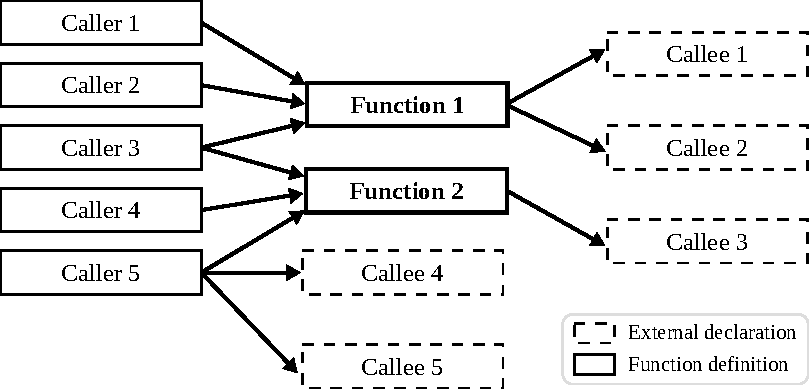
\includegraphics[scale=0.6]{figs/our-cost-model-callgraph-1.pdf}
  \caption{Extracted code without function merging.}
  \label{fig:our-cost-model-callgraph-1}
\end{subfigure}
\begin{subfigure}{0.45\textwidth}
\centering
  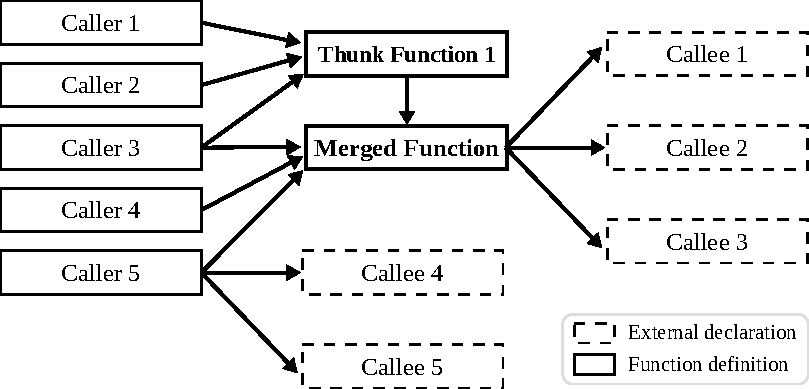
\includegraphics[scale=0.6]{figs/our-cost-model-callgraph-2.pdf}
  \caption{Extracted code with function merging.}
  \label{fig:our-cost-model-callgraph-2}
\end{subfigure}
\caption{Example of the code extracted to compare the binary size before and after function merging, in order to decide whether or not it is profitable to merge a given pair of functions.}
\label{fig:our-cost-model-callgraphs}
\end{figure}

After compiling and measuring the size of the extracted code, we then apply the changes caused by merging the given pair of functions, as illustrated in Figure~\ref{fig:our-cost-model-callgraph-2}.
These changes represent the real impact function merging would cause in the real program.
Once the function merging has been applied, the code is recompiled.
If function merging produces a smaller binary, then these changes are also applied to the real program.
%As shown in Figure~\ref{fig:our-cost-model-callgraph-2}, when applying function merging to the extracted code, it is able to 

\subsection{Learning a Profitability Model}

\begin{figure}[h]
  \centering
  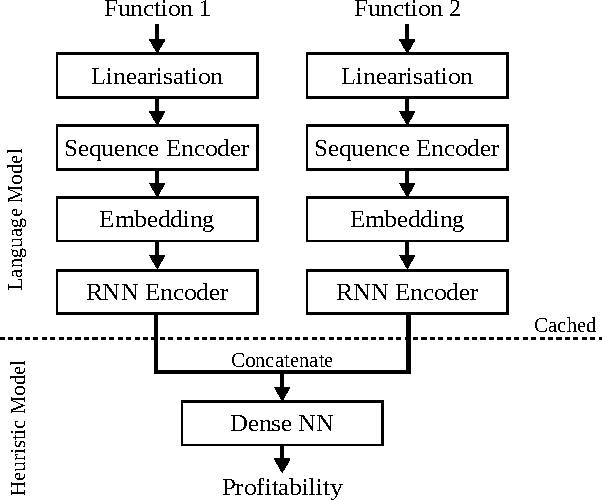
\includegraphics[width=0.45\textwidth]{figs/deeplearning-architecture.pdf}
  \caption{
      The proposed deep-learning model architecture that predicts which pairs of functions will be profitably merged. Code properties are extracted from each function into \textit{context vectors} by the language model.
      These context vectors are cached to be later fed to the heuristic model to produce the final profitability prediction.}
  \label{fig:heuristic-model-architecture}
\end{figure}

Figure~\ref{fig:heuristic-model-architecture} provides an overview of the prediction mechanism.
Our mechanism follows a similar approach to previous deep-learning techniques for tuning compilers~\cite{cummins17, mendis19}.

The same linearised functions used for the merge operations, as described in Chapter~\ref{chp:fm-operation}, are used as input to the prediction model.
First, we use a language model based on recurrent neural networks to encode the input functions into context vectors of fixed size.
These vector encodings can be computed only once per function an cached.
Finally, the context vectors of two input functions are concatenated and fed to a feed-forward neural network that classifies whether or not those functions are profitably merged.


\subsubsection{\textit{inst2vec} Language Model}

\begin{figure}[h]
  \centering
  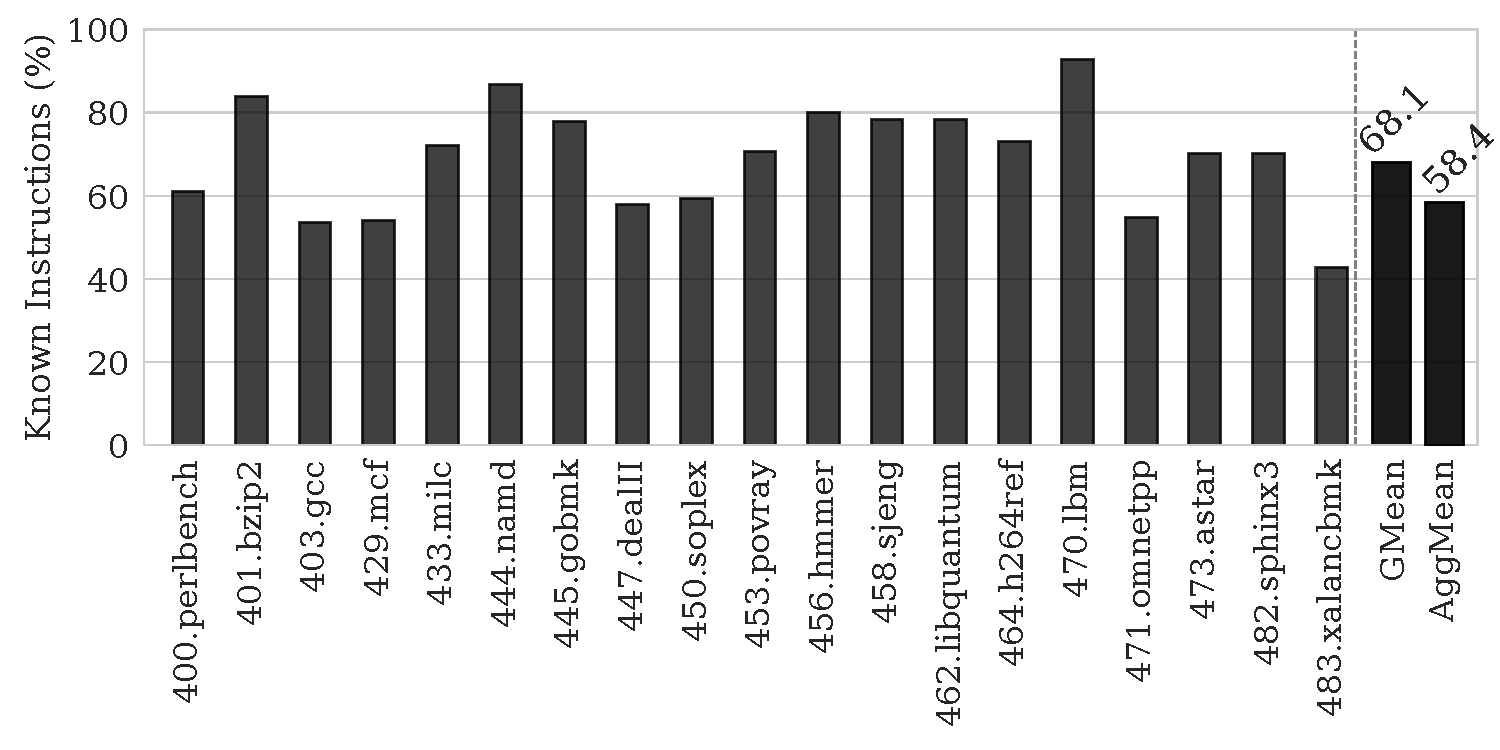
\includegraphics[width=0.45\textwidth]{figs/inst2vec-known.pdf}
  \caption{Percentage of instructions in the pre-trained \textit{inst2vec} language model.}
  \label{fig:inst2vec-known}
\end{figure}

\subsection{Search Strategy}


\begin{figure}[h]
  \centering
  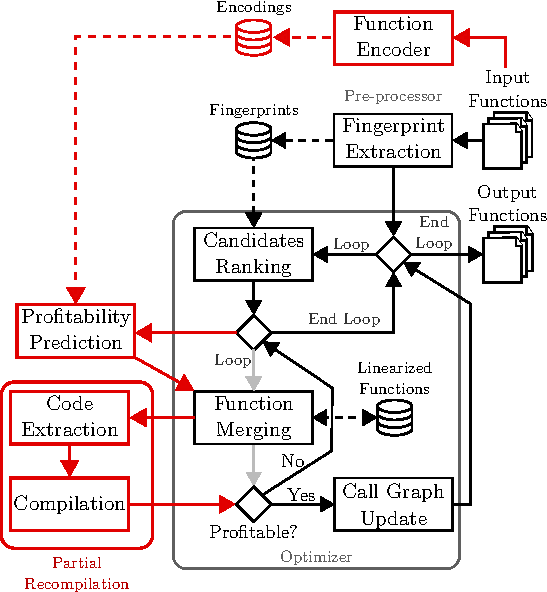
\includegraphics[width=0.45\textwidth]{figs/func-merge-opt-new-arch.pdf}
  \caption{Overview of our extended exploration framework..}
  \label{fig:func-merge-opt-new-arch}
\end{figure}

